\documentclass[manual-fr.tex]{subfiles}
\begin{document}

Pour annoter des documents avec le nouveau modèle, il faut alors sélectionner la chaîne de prétraitement «~NER-retrained.xml~» puis cliquer sur le bouton «~launch SEM~» comme illustré dans la figure \ref{fig:train_sem-07}. Une fois le traitement effectué, SEM indiquera où trouver les fichiers annotés comme illustré dans la figure \ref{fig:train_sem-08}.

\begin{figure}[ht!]
    \begin{center}
    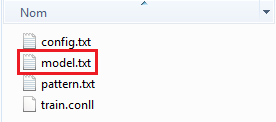
\includegraphics[scale=0.5]{fr/images/train_sem-07.png}
    \end{center}
    \caption{Encadré en rouge : le fichier modèle à copier dans le dossier «~\$\{SEM\_DATA\}/resources/models/fr/NER~»}
    \label{fig:train_sem-07}
\end{figure}

\begin{figure}[ht!]
    \begin{center}
    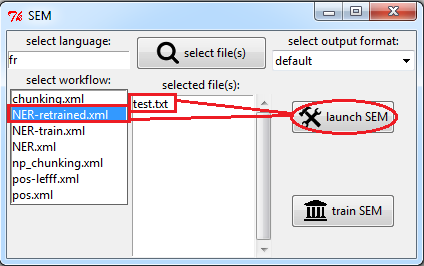
\includegraphics[scale=0.5]{fr/images/train_sem-08.png}
    \end{center}
    \caption{Encadrés en rouges : la chaîne de traitement à utiliser pour annoter avec le nouveau modèle et les fichiers à annoter. Entouré en rouge : le bouton pour lancer l'annotation avec SEM.}
    \label{fig:train_sem-08}
\end{figure}

\end{document}
